In 1982, a new neutral-beam injection heating system was install in the ASDEX tokamak, which pushed the device into a new realm.
A new level of energy confinement time was achieved, measured to be a factor of 2 or more than what was expected.
This state of operation was coined the high-confinement (H--) mode, and is now considered necessary for the future of nuclear fusion as an energy source \cite{arnoux_how_2009} \cite{wagner_development_1984}.
With this new level of energy confinement, the community got one step closer to economic fusion power plants.
The details of this transition, however, are not fully understood.

\section{Characteristics of L-- and H--Mode}\label{sec:characteristics}
Transport of particles and energy in tokamaks has been discovered to be significantly dominated by anomalous (turbulent) transport, which is generally assumed to be generated by turbulence, which are driven by micro-instabilities.
Low-confinement mode, referred to as L--mode, is dominated by this transport at the edge.
The formation of H--mode is due to the suppression of this turbulent transport at the edge of the plasma.
This mode is therefore categorized as having a transport barrier.
The plasma edge is defined to be the thin boundary layer of the plasma just inside the separatrix.

\begin{figure}[tb] % L--H-modes compare
\begin{minipage}{0.49\linewidth}
	\centering
	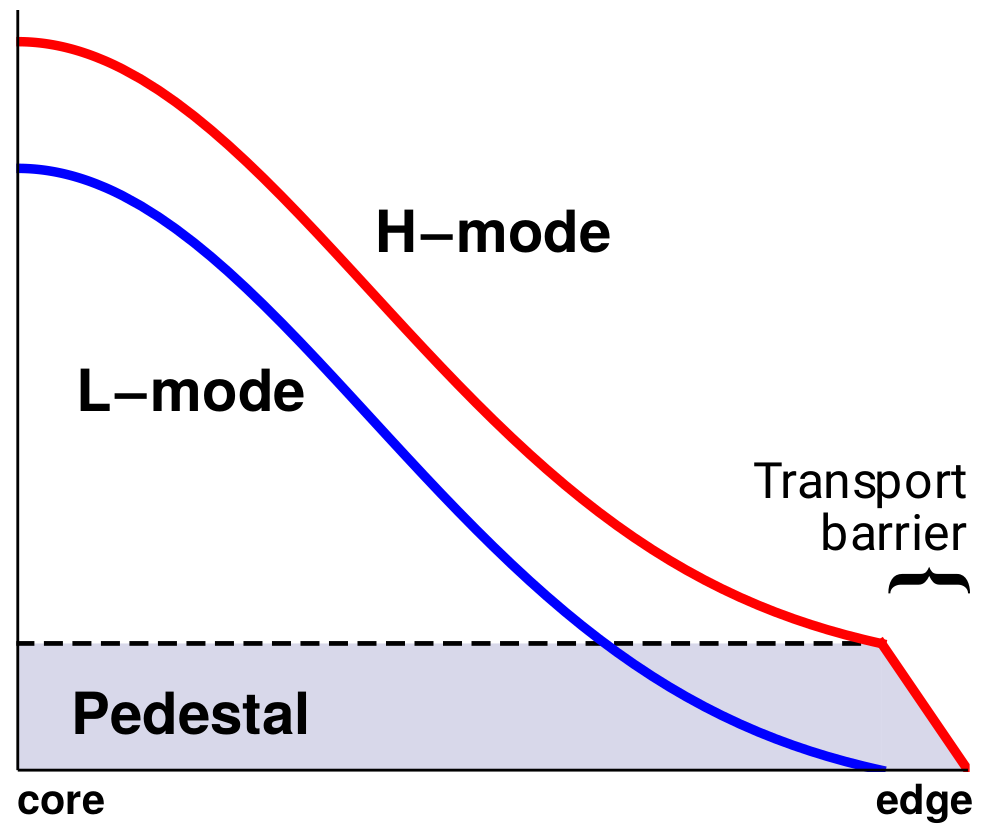
\includegraphics[width=0.8\textwidth]{../Graphics/L-mode_H-mode_compare.png}
\end{minipage}
\hfill
\begin{minipage}{0.49\linewidth}
	\caption{A comparison of the radial pressure profiles of L--mode and H--mode.
	The profile of H--mode can be thought of as on a ``pedestal,'' in which the pressure profile is increase in the core.
	This is due to the transport barrier that is formed at the edge \cite{weymiens_bifurcation_2014}.}
	\label{fig:L-mode_H-mode_compare}
\end{minipage}
\end{figure}

One of the properties of H--mode is its significantly-raised pressure profile compared to that of L--mode, and is said to sit on a ``pedestal.''
Accordingly, there is a steep gradient in the pressure at the edge of the plasma, shown and compared to L--mode in Figure~\ref{fig:L-mode_H-mode_compare} \cite{weymiens_bifurcation_2014}.
This allows for an increased temperature in the core.

In addition, hysteresis is present between the modes, in which the threshold power for the transition between the two modes is based on the current mode.
This is covered in-depth in Section~\ref{ssec:hysteresis}.

\section{The L--H Transition}\label{sec:the_transition}
The key feature that determines a divertor tokamak's operational mode is the amount of external heating power.
Limiter tokamaks are relegated to stay in L--mode, as H--mode is an exclusive operating mode of tokamaks with divertors.
The transition has been observed to occur in one of three manners: sharp, smooth, and oscillatory.

\subsection{Bifurcation Theory}\label{ssec:bif_theory}
A defining feature of L--H transitions is that they can occur very suddenly (the so-called sharp transition), which is characteristic of fold bifurcation behavior.
Mathematically, a bifurcation is defined to be a topological or qualitative change in a system when a small and smooth change of a parameter is made.
A simple example for a fold bifurcation is the following, with $a$ representing the parameter:
\begin{equation} % Simplest fold bifurcation
	\frac{\text{d}x}{\text{d}t} \,=\, \dot{x} \,=\, a + x^2.
	\label{eq:simple_fold}
\end{equation}
This equation can behave in one of three manners:
If $a > 0$, there are no real points of equilibrium, also known as steady-state solutions.
For $a = 0$, there is one equilibrium point at $x = 0$, and two for $a < 0$, at $x = \pm\sqrt{-a}$.
Varying $a$ from some positive real number to some negative number, the fundamental behavior of the solutions changes drastically at $a = 0$ with the sudden appearance of a steady-state solution.
Equation~\ref{eq:simple_fold} is the simplest known form of a fold bifurcation, also known as the saddle-node bifurcation.
The simplest form for any dynamical system is known as the topological norm form.
A parameter plot of $x$ versus $a$ in Fig.~\ref{fig:simple_fold} illustrates this.

%{{{ Two figures for simple bifurcations (co-dimension 1 and 2)
\TwoFig{../Graphics/Bif_Graphs/Simple_fold.png}
	{Plot of parameter space for $\dot{x} = a + x^2$ (Eq.~\ref{eq:simple_fold}), with the co-dimension 1 bifurcation occurring at $a = 0$. %
	For $a < 0$, the system has two steady-state solutions; the green is stable, while the red is unstable.
	For $a > 0$, there is no steady-state solution.}
	{fig:simple_fold}
	{../Graphics/Bif_Graphs/co-2_fold.png}
	{Plot of parameter space for $\dot{x} = -(a + x - x^3)$ (Eq.~\ref{eq:sharp_bif}). %
	This system showcases two fold bifurcations (each of co-dimension 1), at the turning points $a_{\pm\text{crit}}$, with two stable regions, in green and blue. %
	The red region is an intermediate that is unstable.}
	{fig:co-2_fold}
%}}}

The co-dimension of a system refers to the lowest number of parameters required to produce the topological norm form.
Put differently, it is the number of parameters that must be varied for the bifurcation to occur.
In the case of Eq.~\ref{eq:simple_fold}, there is only a single parameter, and is thus referred to as a co-dimension 1 bifurcation \cite{weymiens_bifurcation_2014}.

\subsubsection{Sharp and Smooth Transition Bifurcations}

The dynamic behavior of the L--H transition correspond very closely to a few certain bifurcations.
Sharp and smooth transitions are features of the cusp bifurcation.
The topological norm form of this behavior is
\begin{equation}
	\dot{x} \,=\, -(a + bx - x^3)~.
	\label{eq:sharp_bif}
\end{equation}
Figure~\ref{fig:co-2_fold} is a plot of the parameter space, indicating the stable and unstable steady-state solutions.
This cusp bifurcation can also be regarded as two co-dimension 1 folds, if one can view the positive and negative $x$-domains as separate co-dimension 1 bifurcations.
The distinction between sharp and smooth transitions in this co-dimension 2 bifurcation is solely based on the $b$ parameter, shown in Figure~\ref{fig:hysteresis_b_var}.
As $b$ approaches zero from some positive value, the size of the hysteresis shrinks.

%{{{ Two figures for zeros of the co-dimension 2 bifurcations
\TwoFigOneCap{../Graphics/Bif_Graphs/stationary_b-0_8.png}
	{../Graphics/Bif_Graphs/stationary_b_1_1.png}
	{Phase plots for Eq.~\ref{eq:sharp_bif}, with different values of $a$ within each plot. %
	There is a variance in the number of zeros based on the values of $a$ in the right plot, while there is strictly one zero for all values of $a$ in the left plot. %
	When there is multiple roots, the middle zero is always unstable.}
	{fig:stationaries_b}
%}}}

%{{{ Two figures for complex bifurcations
\TwoFigOneCap{../Graphics/Bif_Graphs/co-2_fold_b_var.png}
	{../Graphics/Bif_Graphs/Bif_3D.png}
	{These plots show the mentioned co-dimension 2 cusp bifurcation, composed of two co-dimension 1 fold bifurcations, as described by Equation~\ref{eq:sharp_bif}.
	The plot on the left shows cross-sections for different $b$ values, with the sharp-smooth boundary occuring at $b = 0$.
	The plot on the right is the surface plot of this same model.}
	{fig:Bif_hysteresis}
%}}}

\subsubsection{Oscillatory Transition Bifurcation}
The third type of transition dynamics in tokamak plasmas is oscillatory, in which the system rapidly oscillates between the two different modes \cite{ryter_survey_2013} \cite{zohm_mhd_1995}.
This phenomenon is referred to by various names, including dithering, I--mode, predator--prey oscillations, and limit cycle oscillations.
It is the most enigmatic of the three discussed, as the least is known about it, and requires a more-complex model than Eq.~\ref{eq:sharp_bif}.

The Hopf, also known as a Poincar\'e-Andronov-Hopf, bifurcation is another co-dimension 1 bifurcation which can describe the oscillatory transition.
It occurs when a periodic solution or limit cycle that surrounds an equilibrium point arises or disappears, when varying the parameter.
Specifically, it occurs where the real part of complex conjugated eigenvalues vanish \cite{munoz-alicea_introduction_2011}.
%{{{ Hopf Bif example and sub/super critical explanation
%When a stable limit cycle encloses an unstable equilibrium point, it is denoted as supercritical.
%For an unstable limit cycle enclosing a stable equilibrium point, it is denoted subcritical.
%The norm form of the bifurcation is as follows,
%\begin{align} % Hopf bifurcation
%	\dot{x} \,=\, x\left((\lambda + i) + b|x|^2\right)~,
%	\label{eq:hopf_bif}
%\end{align}
%with $x$ and $b$ as complex-valued.
%Consider the following polar system, with $a$ as the parameter
%\begin{subequations}
%\begin{align} % Hopf example
%	\dot{r} \,&=\, a r - r^3~, \\
%	\dot{\theta} \,&=\, -1
%\end{align}
%\end{subequations}
%}}}

\begin{figure}[tb] % Co-dimension 3 bifurcation cross-section
\begin{minipage}{0.49\linewidth}
	\centering
	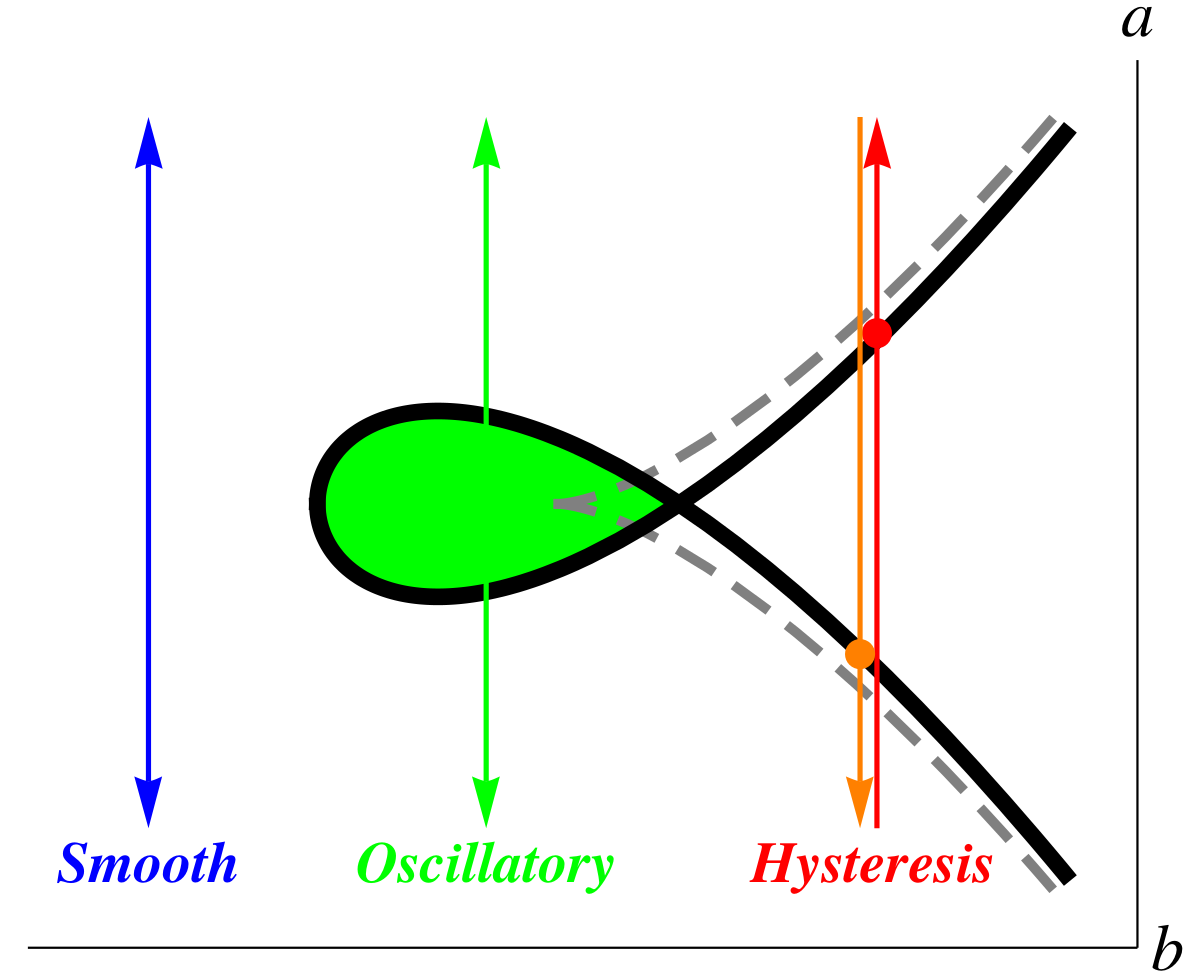
\includegraphics[width=0.9\textwidth]{../Graphics/Bif_Graphs/3_transitions_single_simple.png}
\end{minipage}
\hfill
\begin{minipage}{0.49\linewidth}
	\caption{A parameter plot of the FitzHugh-Nagumo model (Equations \ref{eq:FitzHugh-Nagumo}), a co-dimension 3 bifurcation with the black line indicating the fold bifurcation.
	This model is the one under consideration for accurately describing the L--H transition in tokamak plasmas, with the $b$ parameter dictating the type of transition.
	This $b$ parameter is akin to the density at the edge \cite{weymiens_bifurcation_2014}.}
	\label{fig:co-3}
\end{minipage}
\end{figure}

\subsubsection{Co-dimension 3 Bifurcation}
In order to accurately model to our current knowledge, the oscillatory transition must be incorporated with the sharp and smooth transitions.
Work by Weymiens \cite{weymiens_bifurcation_2014} proves that a ``co-dimension 3 bifurcation robustly connects the three types of transition behaviour'' and investigates using the FitzHugh-Nagumo model.
\begin{subequations}
\begin{align} % FitzHugh-Nagumo model
	\dot{x} \,&=\, a - bx - x^3 + cy~, \\
	\dot{y} \,&=\, -y - x~.
\end{align}
	\label{eq:FitzHugh-Nagumo}
\end{subequations}
This couples the cusp bifurcation to a damped variable, with the coupling parameter $c$.
For as long as $c$ is below some critical value, only the cusp bifurcation will be present; a large enough value gives rise to the oscillatory transition.

All three bifurcations are shown in parameter space in the right plot of Fig.~\ref{fig:Bif_3D_and_co-3}, with the value of the $b$ parameter dictating the type.

\subsection{Hysteresis}\label{ssec:hysteresis}
Hysteresis is a characteristic of any system which the current state of the system depends on its history.
The threshold power for the H--L transition is significantly lower than that of the L--H transition, leading to a region in which there is a non-unique solution to the plasma state.
This requires two separate fold bifurcations each to govern the L--H and H--L transitions separately, which, in turn, requires two types of bifurcation parameters.
The first dictates hysteresis being present in the system; varying this allows for the disappearance of hysteresis when the aforementioned two fold bifurcations merge into a cusp bifurcation.
Varying the second parameter can cause the two stable solutions to be replaced by with unstable solutions, in which the system will oscillate between the solutions.
In the FitzHugh-Nagumo model (Eq.~\ref{eq:FitzHugh-Nagumo}), these are represented by $b$ and $c$, respectively.
\todo{\color{red}{What to do here?}}

\section{Mechanisms}\label{sec:mechanics}
Physically, the L--H transition is a bifurcation in the turbulent transport at the edge of the tokamak.
The prevailing hypothesis for the overarching mechanism for H--mode that can be directly manipulated is that high auxiliary power develops strong sheared plasma flow and suppresses transport \cite{freidberg_plasma_2007}.

\subsection{Turbulence and Sheared Flow Suppression}\label{ssec:turbulence_sheared}
Turbulence is primarily driven by the gradients of the temperature and density, which increase under higher heating.
Drift waves are considered to be the only type of turbulence that pushes radial flux; therefore, it dictates the severity of turbulence and linked transport at the edge of the plasma.
Particular well-known instabilities can be coupled to the drift-wave turbulence, such as the drift resistant ballooning mode, among others \cite{scott_three-dimensional_1997}.
Therefore, a form for the turbulence level will be restricted to one that adheres to the drift wave.

The turbulence evolves as the following, in the absence of sheared flow
\begin{align} % Turbulence ODE
	\frac{\partial\mathcal{E}}{\partial t} \,=\, \gamma_L\mathcal{E} - \alpha_\text{sat}\mathcal{E}^2~.
	\label{eq:turbulence_ode}
\end{align}
This is the result from assuming the particle diffusivity increases linearly with the level of turbulence up to some maximum \cite{diamond_dynamics_1995}.
The first term on the right-hand side is a linear growth term, with $\gamma_L$ as the growth rate, and a nonlinear saturation term, with $\alpha_\text{sat}$ as the saturation rate.
The maximum turbulence is the ratio of the linear growth rate to the saturation rate.

It is now accepted that turbulent transport at the edge is particularly suppressed by sheared flow in the radial direction \cite{terry_suppression_2000}.
The shear stress dissociates smaller turbulent structures, with their energy and momenta transferred to larger flows \cite{staps_backstepping_2017}.

\todo{\color{red}Have fun citing}
Both zonal and mean $\mathbf{E}\times\mathbf{B}$ flows are responsible for the drift wave turbulence.

\subsection{Radial Electric Field}\label{ssec:E_r}
An accepted key mechanism for the transition is the generation of a large radial electric field and the corresponding $\mathbf{E}\times\mathbf{B}$ flows near the edge.
A plethora of individual processes for the generation of such an electric field have been proposed, most of which can be viewed as separate contributions in a radial Poisson's law, with some that tend to reduce the field.
The radial electric field $E_r$ is deduced from the radial force balance for any plasma species $j$, as follows:
\begin{equation}
	E_r \,=\, -\frac{1}{n_j e_j} \frac{\text{d} p_j}{\text{d} r} + V_{\theta j} B_\phi - V_{\phi j} B_\theta
	\label{eq:E_r}
\end{equation}
In the above, $e_j$ represents the charge of the $j$-th species, $n_j$ is the density, $p_j$ is the pressure, and $V_{\theta j}$ and $V_{\phi j}$ are the poloidal and toroidal velocities, respectively.
This grants changes in the radial electric field to be associated with changes in radial gradient of the pressure or either velocities \cite{connor_review_2000}\cite{staps_backstepping_2017}.
However, determining these values is difficult due to large possible error in experiment.

\section{Research Questions}\label{sec:research_questions}
Although there have been compilations of different theories describing the transition, there is yet to be a conclusive, comprehensive one \cite{connor_review_2000}.
There is substantial evidence, both theoretically and experimentally, that a radial electric field is an integral piece in the forming and enforcing of H--mode.
Many of the effects in generating and suppressing the field show up as additive terms in an equation for a radial displacement current.
Because many of these fluxes scale differently, simple scaling laws for H--mode could contrast for regimes where different effects dominate.
It is therefore important to evaluate which terms dominate in their respective regimes before inquiring about global scalings.
The overall problem is thus stated simply: \textbf{Which electric field-generating terms are dominant in concrete experimental tokamak conditions?}
This is in an effort to determine which measurable and controllable values can predict H--mode.

The first consideration is to decide \textbf{which terms should be considered for investigation}, as not all nonambipolar fluxes will significantly contribute to the transition.
For example, the nonambipolar flux due to magnetic ripple loss highly depends on collisionality, in which lower collisionality results in a low flux \cite{stringer_effect_1972}.
Since a relatively ideal operation (temperature on the order of 1 keV at the edge) will be investigated, this flux can be neglected.

\textbf{Identifying what optimal form and relative strengths of each flux and subsequently implementing them} appropriately is the crucial next step.
Because the model is highly nonlinear, it is sensitive to the forms and relative strengths.
The calculation is done with a finite volume method solver, in which the results requires verification with the literature.

The main input heating power regime previously investigate was strictly limited to near the H--L transition \cite{staps_backstepping_2017}.
Performing a scan of input heating power significantly above the lower threshold could show a difference in behavior of the fluxes and resulting field.
Therefore, \textbf{what is the variation in dominance of each field-generating term across increasing input power}, including those inside and outside the regime with non-unique operational modes?

